\documentclass{article}

\usepackage{amsmath, mathrsfs, amssymb, stmaryrd, cancel, relsize,tikz,amsthm}

\theoremstyle{plain}
\newtheorem{theorem}{Theorem}[section]{\bfseries}{\itshape}
\newtheorem{proposition}[theorem]{Proposition}{\bfseries}{\itshape}
\newtheorem{definition}[theorem]{Definition}{\bfseries}{\upshape}
\newtheorem{lemma}[theorem]{Lemma}{\bfseries}{\upshape}
\newtheorem{corollary}[theorem]{Corollary}{\bfseries}{\upshape}
\newtheorem{exercise}[theorem]{Exercise}{\bfseries}{\upshape}

\theoremstyle{definition}
\newtheorem{example}[theorem]{Example}{\bfseries}{\upshape}

\newcommand{\tvs}{\textvisiblespace}
\newcommand{\ra}{\rightarrow}
\newcommand{\la}{\leftarrow}


\title{ITCS 532 Foundations of Computer Science\\
Class 2 - Turing Machine Variants}
\author{Rob Egrot}
\date{}

\begin{document}
\maketitle
\subsection{Multi-tape Turing Machines}
A standard Turing machine has only one tape. We could change the definition so that the machine has two, or even more. Each tape would have its own tape head, though the machine would just have one global state, and the tape heads could move up and down their separate tapes reading and writing independently. Intuitively we might expect that this would give us a more powerful model of computation than single-tape TMs. In other words, that TMs with more than one tape could decide more problems and recognize more languages than their single-tape counterparts. It turns out that this is \emph{not} the case. Multi-tape TMs are equivalent to single-tape TMs, at least as far as decision problems go, in the sense that for any multi-tape TM there's a single-tape TM that gets the same result for the same input. I.e. it will produce the same output, and/or halt in the same state, or run forever if necessary. This is not obvious, but we prove it in theorem \ref{T:multi} below.

\begin{definition}[$k$-tape Turing machine]
A $k$-tape Turing machine $M_k$ is a modified TM with the following additional properties:
\begin{itemize}
\item $M_k$ has $k$ one-way infinite tapes and $k$ independent tape heads. The individual tapes have the same constraints as in the single-tape case.
\item At any moment $M_k$ is in a state $q$. I.e. all tape heads share a single state.
\item We formally describe $M_k$ as a $5$-tuple $(Q,\Sigma,q_0,H,\delta)$. This is just like a normal TM, except that $\delta$ is now defined as 
\begin{equation*}\delta:(Q\setminus H)\times (\Sigma\cup\{\tvs,:\})^k\to Q\times (\Sigma\cup \{\tvs,\la,\ra\})^k\end{equation*}
In other words, $\delta$ has to account for the extra tapes. As in the single-tape case, whenever a tape head reads $:$ the tape head must move right.
\item One tape (call it tape 1) is the designated input tape, and all other tapes are considered to be blank (except for the $:$ symbol at the beginning). The tape heads all start reading the $:$ symbol in the first square of their tape.
\item At each step every tape head reads the symbol on its tape at its position and the tape heads act and the global state changes as determined by $\delta$.
\item Tape 1 is also the output tape. When and if $M_k$ accepts, the output is defined to be the string on tape 1 between $:$ and the first $\tvs$.
\end{itemize}
\end{definition}

\begin{theorem}\label{T:multi}
If $\Sigma$ is a finite alphabet and $M$ is a $k$-tape TM using $\Sigma$ there is a finite alphabet $\Sigma'\supseteq\Sigma$ and a single-tape Turing machine $M'$ using $\Sigma'$ such that for all $x\in \Sigma^*$ we have $M(x)=M'(x)$.  
\end{theorem}
\begin{proof}
The idea is to represent the state of all the tapes, and the positions of all the tape heads, on one tape. To do this we need to expand the alphabet $\Sigma$ considerably. Before we make a formal definition we'll look at an example with two tapes.

\[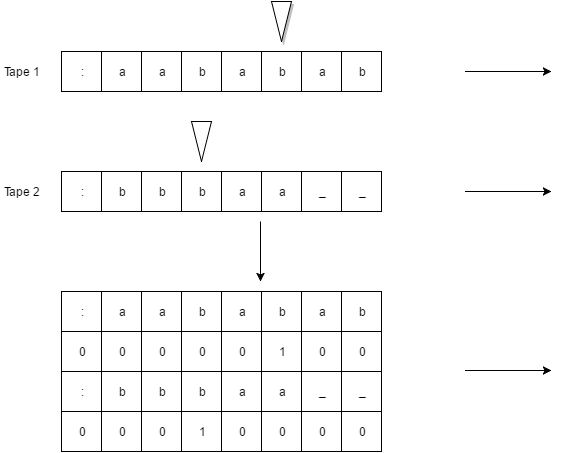
\includegraphics[scale = 0.7]{dMulti.png}\]  

In this example the two tapes of the machine are shown at some point in the run (assume the parts of the tapes out of the picture are blank), along with the positions of the tape heads. The lower part of the picture demonstrates how we would represent this information using only one tape. The symbols of the new tape are represented by the \emph{columns} in the picture. For example, the column 
\[ \left| \begin{array}{c}
b\\1\\a\\0 \end{array} \right| \]
in the 6th position represents that the symbol $b$ is at position 6 on the 1st tape and the 1st tape head is reading that square, and the symbol $a$ is at position 6 on the 2nd tape but the 2nd tape head is somewhere else. 

So, to formally define $\Sigma'$ we need to think about what the possibilities are for the contents of each tape at an arbitrary square, and combine it with the fact that the tape head may or may not be there.  Remember that the very start of the tape contains only the symbol $:$, by definition. The rest of the tape will be used to model the tapes of the multiple tape machine. We will call the start of the tape of single tape machine square -1. We do this because then for $n\geq 0$, square $n$ on the single tape machine corresponds to square $n$ on each tape of the multiple tape machine. In any square other than square 0 (which is a special case as only $:$ can be written there on each tape of the multiple tape machine), there are $|\Sigma\cup\{\tvs\}|$ possibilities for each tape, and for each tape the tape head may or not be present, so we need $(|\Sigma|+1)^k\times 2^k$ symbols to cover all these possible combinations. In addition we need $2^k$ extra symbols for square 0, where only $:$ can be written on each tape but the tape head may or may not be present. Finally we also need every symbol from $\Sigma$ (so that $\Sigma\subset \Sigma'$). So we need $((|\Sigma|+1)^k+1)\times 2^k+|\Sigma|$ symbols in $\Sigma'$.

Anyway, now we know how to represent the state of the tapes of a multi-tape TM using only one tape and an extended alphabet, but we need to work out how to use it simulate the action of the original multi-tape machine. How this works is much too complicated for us to draw using a state change diagram, but we can describe it using high level concepts. So, remember that $M$ is our $k$-tape TM and we are trying to construct a single-tape Turing machine $M'$ using the symbols from $\Sigma'$ so that $M(x)=M'(x)$ for all $x\in \Sigma^*$. To make things easier we set $k=2$. The general case has the same logic. Our machine $M'$ works like this (given input $x$):

\begin{enumerate}
\item $M'$ scans the input $x$ and rewrites $x$ using composite symbols. E.g. $aba\tvs$ will become 
\[ \begin{array}{cccc}
: & a & b & a  \\
1 & 0 & 0 & 0 \\
: & \tvs & \tvs & \tvs  \\
1 & 0 & 0 & 0 
\end{array} \] 
The tape of  $M'$ now represents the initial configuration of $M$ with input $x$. 
\item $M'$ scans the tape till it finds the 1 representing the position of the first tape head. $M'$ changes state to record the symbol the 1st tape head would be reading. $M'$ needs many more states that $M$ to do this, as it must `remember' the state $M$ should be in, and also the current symbol being read by every tape head, and also execute its own program.
\item $M'$ scans the tape for the 1 representing the position of the 2nd tape head and changes state to record the symbols written on the first and second tapes at the appropriate places. 
\item Based on the recorded information about the current symbols being read and the simulated state of $M$ (which $M'$ stores via its own state), $M'$ rewrites the tape to represent $M$ acting on all its tapes.
\item Steps 2, 3, and 4 repeat till $M$ would enter a halting state (if this ever happens!), at which point we proceed to either 6 or 7, depending on the kind of halting state:
\item (Acceptance) $M'$ rewrites the tape so that the output as written on the top row of the combined tape is now written using symbols from $\Sigma$ (so it matches the output of $M$). 
\item (Rejection) $M'$ enters a rejection state.
\end{enumerate}     
\end{proof}

\begin{exercise}
Why is it easy to model a single-tape TM using a multi-tape machine?
\end{exercise}
     


\subsection{The Church-Turing Thesis}
Adding extra tapes is not the only way we can try to extend Turing machines, but it turns out that it's (probably) impossible to design a machine more powerful (in the sense of being able to solve decision problems) than a Turing machine without going beyond the bounds of algorithmic methods. This only applies to situations where you don't care about how long the machine takes. You can design TM variants that can solve problems \emph{faster} than regular TMs, but you can't (it seems) design one capable of solving problems that regular TMs can't. Let's look at some examples.

\begin{example}[Turing machines with a two-way infinite tape] The tape of a regular TM is only infinite in one direction. What if we modified the definition to allow the tape to be infinite in both directions? Would this be a more powerful model of computation? It turns out no. This is fairly easy to see if you think about the multi-tape example. A two-way infinite tape with only one head is at most as powerful as a TM with two tapes and two tape heads. But we saw that this has the same power as a regular TM. Since a TM with a two-way infinite tape is certainly not \emph{less} powerful than a regular TM, they must be equivalent. 
\end{example}

\begin{example}[Turing machines with more than one tape head] We could modify the definition of a Turing machine so that there are two (or more) tape heads working on the same tape. This is slightly tricky to formally define because we have to deal with the possibility of the heads writing in the same space at the same time, but would it give us more power? Again, no. It turns out we can simulate a multi-head TM using a regular TM in a similar way to how we simulated the multi-tape TM. For example, we add symbols to the language so we can model the tape and the positions of the various tape heads on a single tape. For example:

\[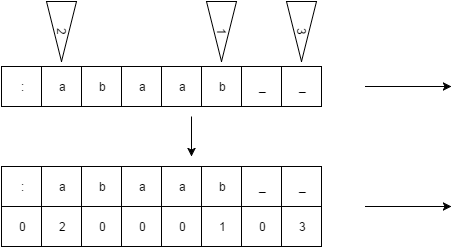
\includegraphics[scale = 0.5]{dMH.png} \]    
\end{example}

\begin{example}[Turing machines operating on a grid] How about instead of a tape we have an infinite grid that the tape head moves around on in two dimensions? Again this is not more powerful. To see this we first model the 2D grid as a sequence of squares in one dimension. This is similar to how we showed the rational numbers are countable. Then we have to create enough states and design the code well enough to deal with the fact that moving the tape head is more complicated now. It's tricky but it can be done.
\end{example}

\begin{exercise}
Prove that the rational numbers $\mathbb{Q}$ are countable.
\end{exercise}

\begin{example}[Turing machines with infinite states] Regular Turing machines can only have a finite number of states. How about if we allow the machine to have an infinite number of states? It turns out that yes, this is more powerful. In fact it's too powerful! If we're allowed to use an infinite number of states then every language over a countable alphabet can be decided by a TM. This is because with an infinite number of states we can have one unique state for every possible input, so all we have to do to `decide' a language is assign acceptance or rejection to each state appropriately. Having an infinite number of states is cheating though, because it's going beyond the realms of computation and into the realm of magic where we can just `guess' the correct answer without having to solve the problem with an algorithm at all.   
\end{example}

People have thought about this very hard, and for a long time, but no one has been able to find a problem for which there is an algorithmic solution that couldn't be abstractly modeled by Turing machines. This leads us to:
\newline
\newline

\begin{centering} \textbf{The Church-Turing Thesis}


\emph{Any problem expressible in a formal language that is solvable by a well-defined step by step procedure can be solved by a Turing machine} \end{centering}
\newline

`Thesis' here is used to mean ``A statement or theory". This is the argument of Alonzo Church. It's impossible to formally prove it, but it would be possible to disprove it by producing a counterexample (though how would you check that your step by step procedure for this hypothetical problem was correct?). Most computer scientists believe that no such counterexample exists. This is a very important idea, because it means that every task you can do with a computer you can, in theory, do with a sufficiently complex Turing machine. Equivalently, any task you can't do with a Turing machine is impossible to do with a computer. So the Church-Turing Thesis, assuming it's true, lets us use the theory of Turing machines to put hard theoretical limits on what can be done with real world computers.




\subsection{Enumerators}
Recall that a formal language $L$ is defined to be recursively enumerable if there is a Turing machine that accepts when given words from $L$ as input, and does not halt for other inputs. \emph{Enumerable}, on the other hand, is a word for something that can be counted, so a \emph{recursively enumerable} language should, logically, be one that can be counted (put into a list) by a recursive procedure. But the standard definition of an r.e. language doesn't say anything about lists or counting. It turns out that these definitions are equivalent though, in a way we make precise below.

\begin{definition}[Enumerator]
An enumerator is a special Turing machine with the following properties:
\begin{enumerate}
\item There is no halt state.
\item There is a special state \emph{print}.
\item The machine starts by erasing the input (or we just assume the input is always empty).
\item When the machine enters the \emph{print} state the current contents of the tape between $:$ and the first $\tvs$ is `printed' (added to the end of an abstract list that starts empty).
\end{enumerate}
\end{definition}  
Enumerators capture the intuitive idea of generating a list using an automated procedure. Given a finite alphabet $\Sigma$, and an enumerator $E$ using $\Sigma$, the set of words that will eventually be printed by $E$ form a subset of $\Sigma^*$, in other words it is a formal language. It turns out that every language created using an enumerator is r.e., and every r.e. language has an enumerator that generates it. This is not obvious, so we prove it as theorem \ref{T:enum} now.

\begin{theorem}\label{T:enum}
Let $\Sigma$ be a finite alphabet and let $L\subseteq\Sigma^*$. Then $L$ is recursively enumerable if and only if there is an enumerator $E$ with the following properties:
\begin{enumerate}
\item If $s\in L$ then $E$ will print $s$ after a finite number of operations.
\item If $E$ prints $s$ then $s\in L$.
\end{enumerate}
\end{theorem}
\begin{proof}
We start by proving that if an enumerator $E$ exists for $L$ then $L$ is r.e. as this is relatively easy. We want to use the enumerator $E$ to build a Turing machine $T_E$ that accepts for all words in $L$, and fails to halt for all other words. Again this is too complicated to draw a state diagram for, so we will describe how the machine works at a higher level. 

We can assume that $T_E$ has multiple tapes, as we know from theorem \ref{T:multi} that if a multi-tape TM exists we can build a single-tape machine. So, $T_E$ stores the input string on one tape, and on another tape it outputs strings as produced by $E$. Every time a new string is produced, $T_E$ compares it to the input string. If they are the same it accepts. Since $E$ is an enumerator for $L$, if the input string is in $L$ it will eventually be produced by $E$, and so $T_E$ semidecides $L$ as required.

The converse is more difficult. We start with a TM $T$ that semidecides a language $L$ (i.e. it accepts on input from $L$, and fails to halt otherwise). We want to use this to create an enumerator $E_T$ that lists the elements of $L$. The basic idea is that $E_T$ will write the strings from $\Sigma^*$ one by one on a tape (again we can safely assume multiple tapes). Every time a new string is written $E_T$ runs $T$ on that string. If $T$ accepts then $E_T$ `prints' the string. So the flow would be something like this:

\[\includegraphics[scale = 0.5]{dEnum.png} \]  

Unfortunately there's a problem. $T(x)$ may not halt! So as soon as we get a string not in $L$ our machine $E_T$ will get stuck and will run forever without printing again. To get around this we have to use a very important technique called \emph{dovetailing}. The modified action of $E_T$ is as follows

\begin{enumerate}
\item Generate a new string $x_1$.
\item Simulate $T(x_1)$ for one step only.
\item Generate a new string $x_2$.
\item Simulate $T(x_1)$ for one more step, then simulate $T(x_2)$ for one step.
\item Generate a new string $x_3$.
\item Simulate $T(x_1)$ for one more step, then simulate $T(x_2)$ for one more step, then simulate $T(x_3)$ for one step.
\item And so on...
\item Whenever $T(x_n)$ succeeds print $x_n$. 
\end{enumerate}
This works because even if one or more of the computations never halts it doesn't matter. Because we add an extra string every cycle, the strings that $T$ doesn't accept don't stop the other strings from getting attention. We know that, for all values of $x$, we will eventually have simulated $T(x)$ for any given number of steps. It might take a long time, but if $T$ accepts $x$ then $E_T$ will notice and print $x$. 

Of course, we have to manage all this using Turing machine architecture, but we have lots of tapes at our disposal. We have one set of tapes for writing all the strings from $\Sigma^*$ (we just pick an order for the symbols in the alphabet, then we can print out all the strings of length one in `lexicographic order', then all the strings of length two and so on). We can easily use a single tape to store all the strings we're currently simulating $T$ on; we just need a special symbol to separate them, and also a way of recording where the simulated tape head currently is, and which state $T$ is supposed to be in, for each computation. 
\end{proof}


\end{document}